% Created 2022-02-25 Fri 17:47
% Intended LaTeX compiler: pdflatex
\documentclass[11pt,a4paper]{article}
\usepackage[utf8]{inputenc}
\usepackage[T1]{fontenc}
\usepackage{fixltx2e}
\usepackage{graphicx}
\usepackage{longtable}
\usepackage{float}
\usepackage{wrapfig}
\usepackage{rotating}
\usepackage[normalem]{ulem}
\usepackage{amsmath}
\usepackage{textcomp}
\usepackage{marvosym}
\usepackage{wasysym}
\usepackage{amssymb}
\usepackage{hyperref}
\usepackage{mathpazo}
\usepackage{color}
\usepackage{enumerate}
\usepackage{lastpage}
\definecolor{bg}{rgb}{0.95,0.95,0.95}
\tolerance=1000
            \usepackage[danish]{babel}

\linespread{1.1}
\hypersetup{pdfborder=0 0 0}

\setlength{\parindent}{0pt}
\usepackage{fancyhdr}
\usepackage{lipsum}
\fancyfoot{}
\pagestyle{fancy}
\rfoot{Page \thepage \hspace{1pt} of \pageref{LastPage}}
\author{Aksel Mannstaedt}
\date{}
\title{Virkeligt hurtige Fourier Transformationer}
\hypersetup{
 pdfauthor={Aksel Mannstaedt},
 pdftitle={Virkeligt hurtige Fourier Transformationer},
 pdfkeywords={},
 pdfsubject={},
 pdfcreator={Emacs 29.0.50 (Org mode 9.6)}, 
 pdflang={Danish}}
\begin{document}

\maketitle
\noindent\rule{\textwidth}{0.5pt}
\begin{center}
Kode med tekst og grafer - \url{https://nbviewer.org/github/unic0rn9k/fourier-notebook/blob/master/README.ipynb}

github repo - \url{https://github.com/unic0nr9k/fourier-notebook}
\end{center}

\noindent\rule{\textwidth}{0.5pt}

\setcounter{tocdepth}{2}
\tableofcontents
\newpage

\section{Teori}
\label{sec:org226d80c}
\subsection{Rekursion og funktionel programmering}
\label{sec:orge5784a7}

Rekursion er helt simpelt, en funktion der kalder sig selv.
Dette bliver brugt meget i funktionel programmering.

Funktionel programmeringssprog er et paradigme kendetegnet ved
et fokus på funktioner i stedet for objekter og kontrol strukturer. \footnote{\url{https://en.wikipedia.org/wiki/Functional\_programming}}

\bigskip

Fordele ved funktionelle programmeringssprog er at de er designet til at formindske side effects,
og derved uforudventet adfærd.
Side effects er defineret som en operation der muterer data udenfor den funktion der ejer data'en.
Dette vil altså siges, at hvis man har en funktion der tager en pointer til en værdi og så ændrer på
den værdi via pointeren, vil det være en side effect af funktionen.

Dette kan skabe uforudventet adfærd i et program og vil derfor typisk gerne undgås.

Fuldkommen funktionelle programmeringssprog er sprog, hvor man ikke kan mutere data overhovedet.
Det betyder altså, at hvis man for eksempel vil lave et for loop, er man nødt til at bruge rekursion.

Fuldkommen funktionelle programmeringssprog bliver ikke rigtigt anvendt i praksis,
men de er dog stadig relevante at skrive om, da de er tættere på matematisk notering
end traditionelle programmeringssprog.

I min case har jeg anvendt fuldkommen funktionel psudo kode til at lave en model
for hvordan jeg ville strukturere min implementering af Cooley-Tukey FFT algoritme.

\subsection{Hvad er en Fourier transformation?}
\label{sec:orga5eb82b}
\newpage

En Fourier transformation er en funktion der tager et polynomium, repræsenteret som en koefficient-vektor,
og transformerer den til en punkt-vektor repræsentation. Dette bliver også kaldt for en time to frequency -domain transformation,
da den også kan repræsenteres som en transformation af bølger repræsenteret som intensitet over tid til intensitet over frekvens.
Jeg vil primært fokusere på bølge repræsentationen af fourier transformationen, der jeg synes den er lidt nemmere at forstå.

Her er som eksempel en bølge og dens tilhørende fourier transformation.
Bølgen er en kombination af en 10Hz bølge og en 25Hz bølge.

\begin{center}
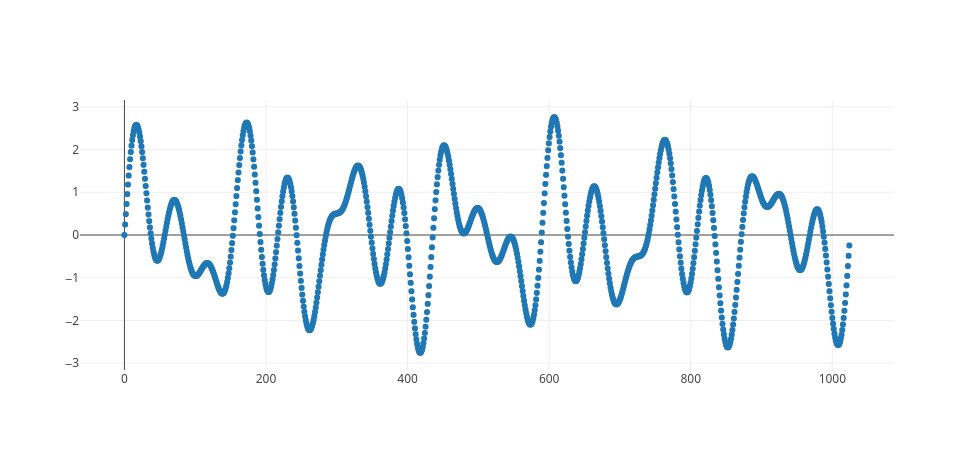
\includegraphics[width=.9\linewidth]{./source_plot2.png}
\end{center}

Her kan man altså se der ligger to top punkter lige omkring 10 og 25 på x-aksen.
\begin{center}
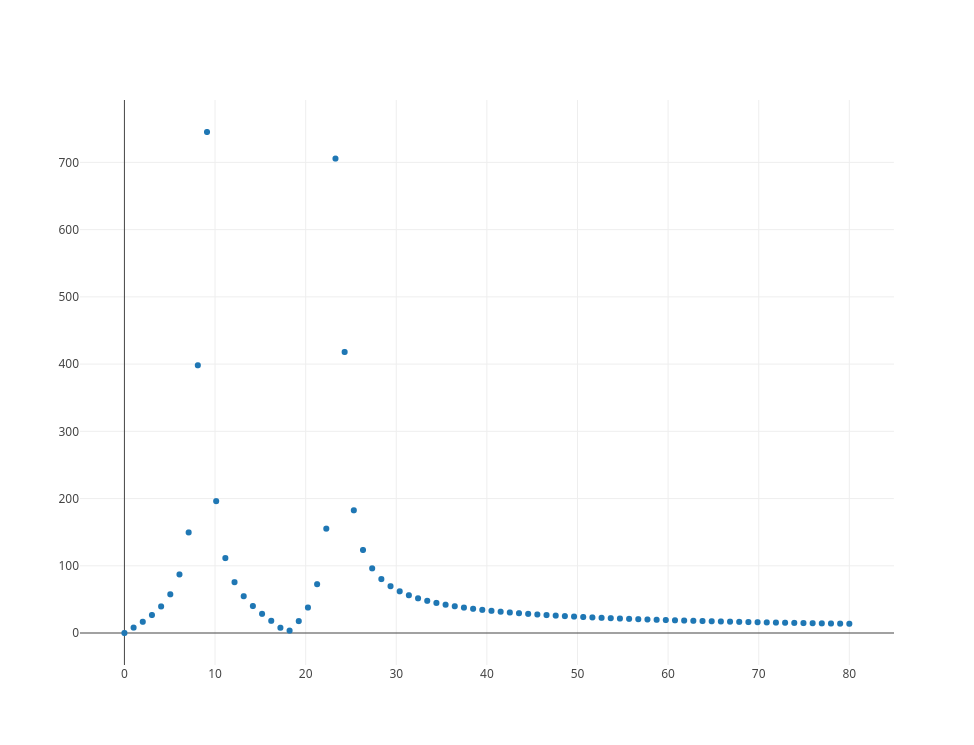
\includegraphics[width=.9\linewidth]{./plot2.png}
\end{center}

\bigskip

\subsection{DFT}
\label{sec:org3737c4e}
DFT er kort for diskret fourier transformation, og var den originale formel opdaget af Joseph Fourier i 1830.
Han fandt ud af, hvordan man kunne lave de her transformationer, før man kunne udregne dem på computere,
eller havde nogen praktisk anvendelse til dem\footnote{\url{https://en.wikipedia.org/wiki/Joseph\_Fourier}}.

Her er f frekvens, t er tid, g er en sammensat bølge funktion og \(\hat{g}\) er den Fourier transformerede funktion af g.
$$
\hat{g}(f) = \int_{+\infin}^{-\infin{}} g(t) \cdot e ^{-2\pi ift}dt
$$

Formlen ovenfor viser hvordan en diskret fourier transformation kan udregnes,
den kan se lidt skræmmende ud, men er nem nok at forstå når man lige har styr på et par koncepter indenfor matematik.

\bigskip

\subsubsection{Komplekse tal og Euler's identitet}
\label{sec:org81c5dd9}

Et komplekst tal er et tal bestående af en imaginær del og en reel del (summen af dem).
Den imaginære del af det komplekse tal er defineret som produktet af et
virkeligt tal og \(i\).

\(i\) er defineret som kvadratroden af -1. (altså det findes ikke).

Det giver måske ikke lige umiddelbart så meget mening, men en nem måde at tænke på det,
er som en 2d vektor der har nogen specielle regne regler.

For eksempel vil \((0 + 1i)^2\) være -1, da \(i^2\) skal give -1.

Komplekse tal bliver typisk også visualiseret som en 2d-vektor,
hvor den reelle del er på x-aksen, og den imaginære del er på y-aksen.

Her vil det svares til en \(90^\circ\) rotation, i det komplekse plan, at gange med \(i\).

$$
(1 + 0i) \cdot i = 0 + 1i
$$
$$
(0 + 1i) \cdot i = -1 + 0i
$$
$$
(-1 + 0i) \cdot i = 0 - 1i
$$
osv\ldots{}

\newpage

For at kunne forstå fourier transformeringer er det vigtigt at forstå Euler's identitet,
som er defineret som

$$
e^{\pi i} = -1
$$

Dette udtryk kommer af at \(e^x\) er sit eget derivativ (\(e\) er Euler's konstant \footnote{\url{https://en.wikipedia.org/wiki/Euler\%27s\_constant}}),
det vil altså siges at \(\frac{d}{dx}e^{kx} = k\cdot e^{kx}\), hvor k er en konstant.

Altså man kan sige at \(e^{kx}\) bevæger sig i retningen \(k \cdot e^{kx}\).
Det betyder at hvis vi bytter \(k\) ud med \(i\), må \(e^{ix}\) bevæge sig mod en \(90^\circ\) rotation med en hastighed af en radian per x.

Her vil en halv rotation derfor svare til \(x=\pi\) og vi kan derved konkludere at \(e^{\pi i} = -1\).

\subsubsection{Uddybning af Fourier transformation}
\label{sec:org30372c5}

Den innerste del af den diskrete fourier transformering kan ses lidt som et prik produkt
$$
f(t) = g(t) \cdot e ^{-2\pi ift}
$$

Her vil det virkelige komponent af \(f(t)\) være støre når intensiteten af \(g(t)\)
matcher den der ville findes hvis frekvensen af \(g\) var \(f\).

Dette kan intuitivt forstås, som at når \(t\) værdier ligger i bølgedale, vil \(e^{-2\pi ift}\) være negativ
og derfor vil \(f(t)\) være positiv hvis \(g(t)\) også er negativ.

\(-2\pi\) sikre at en øgelse af en tidsenhed svarende til en periode frekvensen \(f\) også vil resultere
i en fuld rotation af \(e^{-2\pi ift}\).

\subsection{FFT}
\label{sec:org54614df}

\subsubsection{Rekursion}
\label{sec:orgc7aa636}

\section{Tooling (programmering)}
\label{sec:orgac6c0cf}
Jeg valgte at skrive koden til denne case i rust, da jeg er komfortabel med sproget,
og gerne ville eksperimentere med at lave en hurtig implementering af Cooley-Tukey algoritmen.

Rust er et rigtigt hurtigt sprog, dette skyldes blandt andet at det bruger llvm som backend,
men også rust's brug af zero-cost-abstractions.

Jeg valgte at skrive koden i en jupyter notebook, da jeg ikke havde nogen egentlig
applikation af min kode i tankerne under forløbet.
Det viste sig også at være super praktisk til at lave tdd (test-driven-developement),
da det betød jeg kunne smide nogen grafer ind, og have dem opdateret i næsten realtime,
mens jeg arbejdede på implementeringen af fft algoritmen.

\subsection{Rust sprog paradimer}
\label{sec:orgd957105}
Rust er et memory-safe programmeringssprog,
hvilket betyder at det by-default ikke lader en skrive koder, der kan forudsige undefined-behavior\footnote{\url{https://doc.rust-lang.org/reference/behavior-considered-undefined.html}}

\section{Inplace operationer og statisk allokering}
\label{sec:org70a886b}

\section{Bilag}
\label{sec:org21df03c}
\begin{center}
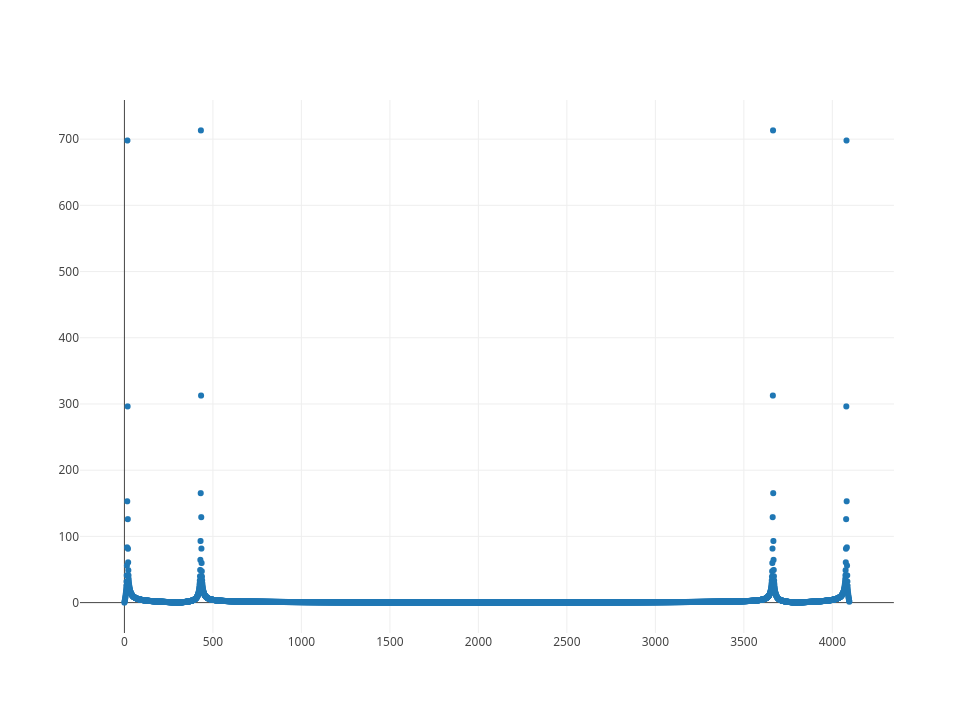
\includegraphics[width=.9\linewidth]{./plot1.png}
\end{center}

\section{Bibliografi}
\label{sec:org8999821}

1: Undefined-behavior - \url{https://doc.rust-lang.org/reference/behavior-considered-undefined.html}

2: Funktionel programmering - \url{https://en.wikipedia.org/wiki/Functional\_programming}

3: Fourier - \url{https://en.wikipedia.org/wiki/Joseph\_Fourier}

4: Euler's konstant - \url{https://en.wikipedia.org/wiki/Euler\%27s\_constant}
\end{document}
